% DMA Session 7: Relationales Modell & Transformation
% 180-Minuten-Block (Vorlesung + Übung interwoven)

\documentclass[usenames,dvipsnames,10pt,aspectratio=169]{beamer}
\usepackage[T1]{fontenc}
\usepackage[utf8]{inputenc}
\usepackage{verbatim}

\usetheme{ims}

\usepackage{booktabs}
\usepackage{multicol}
\usepackage{listings}
\usepackage[table]{xcolor}
\usepackage{graphicx}
\usepackage{tikz}
\usetikzlibrary{shapes.geometric, arrows.meta, positioning, calc, fit, backgrounds, matrix}
\usepackage{pifont}

% ===== CLICKABLE AGENDA WITH PROGRESS INDICATOR =====
\usepackage{hyperref}
\hypersetup{colorlinks=false, pdfborder={0 0 0}}

% Phase counter for progress tracking
\newcounter{currentphase}
\setcounter{currentphase}{0}

% ER-Diagram TikZ styles (from Session 6)
\tikzset{
    entity/.style={rectangle, draw=IMSBlue, fill=IMSBlue!10, thick,
        minimum width=2.5cm, minimum height=1cm, font=\bfseries},
    weakentity/.style={rectangle, draw=IMSBlue, fill=IMSBlue!10, thick,
        minimum width=2.5cm, minimum height=1cm, font=\bfseries,
        double, double distance=2pt},
    relationship/.style={diamond, draw=IMSOrange, fill=IMSOrange!15, thick,
        minimum width=1.8cm, minimum height=1.2cm, aspect=2, font=\small},
    attribute/.style={ellipse, draw=gray!70, fill=gray!10,
        minimum width=1.5cm, minimum height=0.6cm, font=\small},
    card/.style={font=\footnotesize, text=IMSBlue},
    erline/.style={thick, gray!70},
    % Table styles
    tablebox/.style={rectangle, draw=IMSBlue, fill=IMSBlue!5, thick,
        minimum width=4cm, minimum height=0.8cm, font=\ttfamily\small},
    tableheader/.style={rectangle, draw=IMSBlue, fill=IMSBlue!20, thick,
        minimum width=4cm, minimum height=0.8cm, font=\ttfamily\small\bfseries},
    pkstyle/.style={font=\ttfamily\small, text=IMSBlue},
    fkstyle/.style={font=\ttfamily\small, text=IMSOrange},
    roadmapbox/.style={rectangle, rounded corners, minimum width=3cm, minimum height=1cm,
        text centered, draw=IMSBlue, fill=IMSBlue!10, font=\small\bfseries},
    roadmaparrow/.style={-{Stealth[length=3mm]}, thick, IMSBlue},
    quizbox/.style={rectangle, rounded corners, draw=IMSOrange, fill=IMSOrange!10,
        minimum width=10cm, minimum height=1.5cm, font=\large},
}

% SQL Listing Style
\lstdefinestyle{sql}{
    language=SQL,
    basicstyle=\ttfamily\footnotesize,
    keywordstyle=\color{IMSBlue}\bfseries,
    stringstyle=\color{IMSOrange},
    commentstyle=\color{gray}\itshape,
    showstringspaces=false,
    breaklines=true,
    frame=single,
    backgroundcolor=\color{gray!10},
    morekeywords={SERIAL, BOOLEAN, TEXT, REFERENCES, CONSTRAINT, CASCADE, RESTRICT, PRIMARY, FOREIGN, KEY, UNIQUE, CHECK, DEFAULT, AUTO_INCREMENT, INT, VARCHAR, DATE, DECIMAL, NOT, NULL, NO, ACTION, SET},
    literate={ü}{{\"u}}1 {ä}{{\"a}}1 {ö}{{\"o}}1 {Ü}{{\"U}}1 {Ä}{{\"A}}1 {Ö}{{\"O}}1 {ß}{{\ss}}1
}

\lstset{style=sql}

\newcommand{\cmark}{\textcolor{green!70!black}{\ding{51}}}
\newcommand{\xmark}{\textcolor{red}{\ding{55}}}
\newcommand{\pk}[1]{\underline{\texttt{#1}}}
\newcommand{\fk}[1]{\texttt{\textcolor{IMSOrange}{#1}}}

% Clickable agenda item
\newcommand{\agendaitem}[3]{%
    \ifnum#1=#2
        \textcolor{IMSOrange}{$\blacktriangleright$ \textbf{\hyperlink{phase#2}{#3}}}%
    \else
        \textcolor{gray!70}{\phantom{$\blacktriangleright$} \hyperlink{phase#2}{#3}}%
    \fi\\[0.3em]%
}

% Progress dots for footline (clickable)
\newcommand{\progressdots}{%
    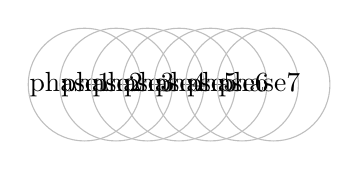
\begin{tikzpicture}[baseline=-0.5ex]
        \foreach \i in {1,...,7} {
            \ifnum\value{currentphase}=\i
                \node[circle, fill=IMSOrange, minimum size=0.24cm, inner sep=0pt] at (\i*0.4,0) {\hyperlink{phase\i}{\phantom{oo}}};
            \else
                \ifnum\value{currentphase}>\i
                    \node[circle, fill=IMSBlue!60, minimum size=0.2cm, inner sep=0pt] at (\i*0.4,0) {\hyperlink{phase\i}{\phantom{oo}}};
                \else
                    \node[circle, draw=gray!50, minimum size=0.2cm, inner sep=0pt] at (\i*0.4,0) {\hyperlink{phase\i}{\phantom{oo}}};
                \fi
            \fi
        }
    \end{tikzpicture}%
}

% Add progress indicator to footline
\setbeamertemplate{footline}{%
    \leavevmode%
    \hbox{%
        \begin{beamercolorbox}[wd=.33\paperwidth,ht=2.5ex,dp=1ex,left]{author in head/foot}%
            \usebeamerfont{author in head/foot}\hspace*{2ex}\insertshortauthor
        \end{beamercolorbox}%
        \begin{beamercolorbox}[wd=.34\paperwidth,ht=2.5ex,dp=1ex,center]{title in head/foot}%
            \progressdots
        \end{beamercolorbox}%
        \begin{beamercolorbox}[wd=.33\paperwidth,ht=2.5ex,dp=1ex,right]{date in head/foot}%
            \usebeamerfont{date in head/foot}\insertframenumber{} / \inserttotalframenumber\hspace*{2ex}
        \end{beamercolorbox}%
    }%
    \vskip0pt%
}

\newcommand{\showagenda}[1]{%
\setcounter{currentphase}{#1}%
\begin{frame}{Agenda}
\hypertarget{phase#1}{}%
\vfill
\begin{center}
\begin{minipage}{0.65\textwidth}
\large
\agendaitem{#1}{1}{1 ~ Rückblick \& Das Relationale Modell}
\agendaitem{#1}{2}{2 ~ Schlüssel im Detail}
\agendaitem{#1}{3}{3 ~ Transformation: 1:N-Beziehungen}
\agendaitem{#1}{4}{4 ~ Transformation: M:N-Beziehungen}
\agendaitem{#1}{5}{5 ~ Transformation: 1:1 \& Sonderfälle}
\agendaitem{#1}{6}{6 ~ CREATE TABLE in SQL}
\agendaitem{#1}{7}{7 ~ Zusammenfassung}
\end{minipage}
\end{center}
\vfill
\end{frame}
}

%%%%%%%%%%%%%%%%%%%%%%%%%%%%%%%%%%%%%%%%%%%%%%%%%%%%%%%%%%%%%%%%%%%%%%%%%%%%%%%%%%%%%
\title[DMA 07]{Datenmanagement \& -analyse}
\subtitle{Vorlesung 7: Relationales Modell \& Transformation}
\author{Prof. Dr. Christoph M. Flath}
\institute{Lehrstuhl für Wirtschaftsinformatik und Business Analytics\\Julius-Maximilians-Universität Würzburg}
\date{Sommersemester 2026}
%%%%%%%%%%%%%%%%%%%%%%%%%%%%%%%%%%%%%%%%%%%%%%%%%%%%%%%%%%%%%%%%%%%%%%%%%%%%%%%%%%%%%

\begin{document}

% ===== TITLE =====
\begin{frame}[plain]
    \titlepage
\end{frame}

% ===== PHASE 1: Rückblick & Das Relationale Modell =====
\showagenda{1}

\begin{frame}{Rückblick: Der Modellierungsprozess}
\begin{center}
\begin{tikzpicture}[node distance=1.2cm, scale=0.85, transform shape]
    \node[roadmapbox, minimum width=2.8cm] (real) {Reale Welt};
    \node[roadmapbox, minimum width=2.8cm, right=of real, fill=green!10, draw=green!50!black] (er) {ER-Modell};
    \node[roadmapbox, minimum width=3.2cm, right=of er, fill=IMSOrange!20, draw=IMSOrange] (rel) {Rel. Schema};
    \node[roadmapbox, minimum width=2.8cm, right=of rel] (sql) {SQL-Tabellen};

    \draw[roadmaparrow] (real) -- (er) node[midway, above, font=\footnotesize] {\cmark};
    \draw[roadmaparrow, IMSOrange, thick] (er) -- (rel) node[midway, above, font=\footnotesize] {Heute!};
    \draw[roadmaparrow] (rel) -- (sql) node[midway, above, font=\footnotesize] {Heute!};
\end{tikzpicture}
\end{center}

\vspace{1em}
\textbf{Letzte Session:}
\begin{itemize}
    \item Entitäten, Attribute, Beziehungen
    \item Kardinalitäten (1:1, 1:N, M:N)
    \item Chen-Notation
\end{itemize}

\textbf{Diese Session:}
\begin{itemize}
    \item ER-Modell $\rightarrow$ Tabellen (Relationales Schema)
    \item CREATE TABLE mit Schlüsseln
\end{itemize}
\end{frame}

\begin{frame}{Das Relationale Modell}
\begin{columns}[T]
\column{0.55\textwidth}
\textbf{Erfinder:} Edgar F. Codd (IBM, 1970)

\vspace{0.5em}
\textbf{Kernidee:} Alle Daten in \textbf{Tabellen} (Relationen)

\vspace{1em}
\textbf{Terminologie:}
\begin{itemize}
    \item \textbf{Relation} = Tabelle
    \item \textbf{Tupel} = Zeile (Datensatz)
    \item \textbf{Attribut} = Spalte
    \item \textbf{Domäne} = Wertebereich einer Spalte
\end{itemize}

\vspace{1em}
\textbf{Beispiel:}\\
Relation \texttt{Spieler} mit 10 Tupeln und 4 Attributen

\column{0.45\textwidth}
\begin{center}
\small
\begin{tabular}{|c|c|c|c|}
\hline
\rowcolor{IMSBlue!20}
\textbf{ID} & \textbf{Name} & \textbf{Pos} & \textbf{Alter} \\
\hline
1 & Müller & Sturm & 35 \\
\hline
2 & Neuer & Tor & 38 \\
\hline
3 & Kimmich & Mittelfeld & 29 \\
\hline
\multicolumn{4}{|c|}{...} \\
\hline
\end{tabular}

\vspace{1em}
\footnotesize
$\uparrow$ Attribute (Spalten)\\
$\leftarrow$ Tupel (Zeilen)
\end{center}
\end{columns}
\end{frame}

\begin{frame}{Eigenschaften einer Relation}
\begin{columns}[T]
\column{0.5\textwidth}
\textbf{Regeln für Relationen:}
\begin{enumerate}
    \item Jede Zeile ist \textbf{eindeutig}
    \item Jede Spalte hat einen \textbf{eindeutigen Namen}
    \item Alle Werte einer Spalte haben \textbf{gleichen Typ}
    \item Werte sind \textbf{atomar} (nicht teilbar)
    \item \textbf{Reihenfolge} der Zeilen/Spalten ist egal
\end{enumerate}

\column{0.5\textwidth}
\textbf{Relationales Schema:}

\vspace{0.5em}
Beschreibung der Tabellenstruktur:

\vspace{0.5em}
\texttt{Spieler(\underline{ID}, Name, Position, Alter)}

\vspace{1em}
\begin{itemize}
    \item Tabellenname
    \item Attribute in Klammern
    \item Primärschlüssel \underline{unterstrichen}
\end{itemize}
\end{columns}

\vspace{1em}
\begin{block}{Notation}
\texttt{Tabellenname(\underline{PK}, Attribut1, Attribut2, \#FK)}
\begin{itemize}
    \item \underline{Unterstrichen} = Primärschlüssel
    \item \# = Fremdschlüssel
\end{itemize}
\end{block}
\end{frame}

\begin{frame}{Vom ER-Modell zum relationalen Schema}
\textbf{Warum diese Transformation?}

\vspace{1em}
\begin{columns}[T]
\column{0.5\textwidth}
\textbf{ER-Modell:}
\begin{itemize}
    \item Konzeptuelles Modell
    \item Für Menschen verständlich
    \item Graphische Notation
    \item Unabhängig vom DBMS
\end{itemize}

\column{0.5\textwidth}
\textbf{Relationales Schema:}
\begin{itemize}
    \item Logisches Modell
    \item Für DBMS umsetzbar
    \item Textbasierte Notation
    \item Direkt in SQL übersetzbar
\end{itemize}
\end{columns}

\vspace{1em}
\begin{center}
\begin{tikzpicture}[scale=0.7, transform shape]
    \node[entity] (e) at (0,0) {Spieler};
    \node[attribute] (a1) at (-2,1.2) {Name};
    \node[attribute, double, double distance=1pt] (a2) at (0,1.5) {\underline{ID}};
    \node[attribute] (a3) at (2,1.2) {Position};
    \draw[erline] (e) -- (a1);
    \draw[erline] (e) -- (a2);
    \draw[erline] (e) -- (a3);

    \node at (4.5,0) {\Large$\Rightarrow$};

    \node[font=\ttfamily\small] at (8,0) {Spieler(\underline{ID}, Name, Position)};
\end{tikzpicture}
\end{center}
\end{frame}

% ===== PHASE 2: Schlüssel =====
\showagenda{2}

\begin{frame}{Schlüssel: Übersicht}
\begin{center}
\begin{tikzpicture}[scale=0.9, transform shape]
    \node[roadmapbox, minimum width=4cm, fill=IMSBlue!20] (super) at (0,3) {Superschlüssel};
    \node[roadmapbox, minimum width=4cm, fill=IMSBlue!30] (kand) at (0,1.5) {Kandidatenschlüssel};
    \node[roadmapbox, minimum width=4cm, fill=IMSBlue!40] (prim) at (-2.5,0) {Primärschlüssel};
    \node[roadmapbox, minimum width=4cm, fill=gray!20] (alt) at (2.5,0) {Alternativschlüssel};

    \draw[roadmaparrow] (super) -- (kand);
    \draw[roadmaparrow] (kand) -- (prim);
    \draw[roadmaparrow] (kand) -- (alt);

    \node[right=0.5cm of super, font=\small, text width=5cm] {Jede Attributkombination, die Tupel eindeutig identifiziert};
    \node[right=0.5cm of kand, font=\small, text width=5cm] {Minimaler Superschlüssel (keine überflüssigen Attribute)};
    \node[below=0.3cm of prim, font=\small] {Der gewählte Schlüssel};
    \node[below=0.3cm of alt, font=\small] {Nicht gewählte Kandidaten};
\end{tikzpicture}
\end{center}
\end{frame}

\begin{frame}{Schlüssel: Beispiel}
\textbf{Tabelle Mitarbeiter:}
\begin{center}
\small
\begin{tabular}{|c|c|c|c|c|}
\hline
\rowcolor{IMSBlue!20}
\textbf{MitarbeiterNr} & \textbf{SVNr} & \textbf{Name} & \textbf{Abteilung} & \textbf{Gehalt} \\
\hline
101 & 12345678 & Müller & IT & 5000 \\
\hline
102 & 23456789 & Schmidt & HR & 4500 \\
\hline
103 & 34567890 & Müller & IT & 5500 \\
\hline
\end{tabular}
\end{center}

\vspace{1em}
\textbf{Analyse:}
\begin{itemize}
    \item \textbf{Superschlüssel:} \{MitarbeiterNr\}, \{SVNr\}, \{MitarbeiterNr, Name\}, \{MitarbeiterNr, SVNr\}, ...
    \item \textbf{Kandidatenschlüssel:} \{MitarbeiterNr\}, \{SVNr\}
    \item \textbf{Kein Schlüssel:} \{Name\} (Duplikat: Müller), \{Abteilung\}, \{Gehalt\}
\end{itemize}

\vspace{0.5em}
\begin{block}{Entscheidung}
Wir wählen \textbf{MitarbeiterNr} als Primärschlüssel $\rightarrow$ \textbf{SVNr} wird Alternativschlüssel
\end{block}
\end{frame}

\begin{frame}{Primärschlüssel (Primary Key)}
\begin{columns}[T]
\column{0.5\textwidth}
\textbf{Definition:}\\
Attribut(e), die jede Zeile \textbf{eindeutig identifizieren}.

\vspace{1em}
\textbf{Eigenschaften:}
\begin{itemize}
    \item \textbf{Eindeutig} -- keine Duplikate
    \item \textbf{Nicht NULL} -- immer ein Wert
    \item \textbf{Stabil} -- ändert sich nicht
    \item \textbf{Minimal} -- keine überflüssigen Teile
\end{itemize}

\vspace{1em}
\textbf{Natürlich vs. Künstlich:}
\begin{itemize}
    \item Natürlich: ISBN, Matrikelnummer
    \item Künstlich: Auto-ID (1, 2, 3, ...)
\end{itemize}

\column{0.5\textwidth}
\begin{center}
\small
\begin{tabular}{|c|c|c|}
\hline
\rowcolor{IMSBlue!20}
\textbf{\underline{ID}} & \textbf{Name} & \textbf{Position} \\
\hline
1 & Müller & Sturm \\
\hline
2 & Neuer & Tor \\
\hline
3 & Müller & Abwehr \\
\hline
\end{tabular}

\vspace{1em}
\footnotesize
``Name'' wäre kein guter PK\\
(zwei Müller möglich!)
\end{center}

\vspace{1em}
\begin{alertblock}{Best Practice}
Im Zweifelsfall: Künstlicher Schlüssel (ID)
\end{alertblock}
\end{columns}
\end{frame}

\begin{frame}{Zusammengesetzter Primärschlüssel}
\textbf{Definition:} Primärschlüssel aus \textbf{mehreren Attributen}

\vspace{1em}
\textbf{Wann nötig?}
\begin{itemize}
    \item Kein einzelnes Attribut ist eindeutig
    \item Beziehungstabellen bei M:N-Beziehungen
    \item Schwache Entitäten
\end{itemize}

\vspace{1em}
\textbf{Beispiel: Buchung}
\begin{center}
\small
\begin{tabular}{|c|c|c|c|}
\hline
\rowcolor{IMSBlue!20}
\textbf{\underline{Flug\_ID}} & \textbf{\underline{Sitz\_Nr}} & \textbf{Passagier} & \textbf{Datum} \\
\hline
LH123 & 12A & Müller & 2026-05-15 \\
\hline
LH123 & 12B & Schmidt & 2026-05-15 \\
\hline
LH456 & 12A & Weber & 2026-05-15 \\
\hline
\end{tabular}
\end{center}

\vspace{0.5em}
\begin{itemize}
    \item Flug\_ID allein nicht eindeutig (mehrere Sitze)
    \item Sitz\_Nr allein nicht eindeutig (mehrere Flüge)
    \item \textbf{Kombination} (Flug\_ID, Sitz\_Nr) ist eindeutig!
\end{itemize}
\end{frame}

\begin{frame}{Fremdschlüssel (Foreign Key)}
\begin{columns}[T]
\column{0.55\textwidth}
\textbf{Definition:}\\
Attribut, das auf den \textbf{Primärschlüssel einer anderen Tabelle} verweist.

\vspace{1em}
\textbf{Zweck:}
\begin{itemize}
    \item Verbindet Tabellen
    \item Stellt Beziehungen her
    \item Erzwingt \textbf{referentielle Integrität}
\end{itemize}

\vspace{1em}
\textbf{Referentielle Integrität:}\\
Ein Fremdschlüssel muss auf einen \textbf{existierenden} Primärschlüssel zeigen.

\column{0.45\textwidth}
\begin{center}
\small
\textbf{Spieler}
\begin{tabular}{|c|c|c|}
\hline
\rowcolor{IMSBlue!20}
\underline{ID} & Name & \textcolor{IMSOrange}{\#Verein\_ID} \\
\hline
1 & Müller & \textcolor{IMSOrange}{1} \\
\hline
2 & Wirtz & \textcolor{IMSOrange}{2} \\
\hline
\end{tabular}

\vspace{0.5em}
$\downarrow$ verweist auf $\downarrow$

\vspace{0.5em}
\textbf{Verein}
\begin{tabular}{|c|c|}
\hline
\rowcolor{IMSBlue!20}
\underline{ID} & Name \\
\hline
1 & Bayern München \\
\hline
2 & Bayer Leverkusen \\
\hline
\end{tabular}
\end{center}
\end{columns}
\end{frame}

\begin{frame}{Referentielle Integrität: Warum wichtig?}
\textbf{Was passiert ohne Integritätsprüfung?}

\vspace{1em}
\begin{center}
\small
\begin{tabular}{|c|c|c|}
\hline
\rowcolor{IMSBlue!20}
\underline{ID} & Name & \textcolor{red}{\#Verein\_ID} \\
\hline
1 & Müller & \textcolor{red}{99} \\
\hline
\end{tabular}

\vspace{0.5em}
$\downarrow$ Verein 99 existiert nicht! $\downarrow$

\vspace{0.5em}
\begin{tabular}{|c|c|}
\hline
\rowcolor{IMSBlue!20}
\underline{ID} & Name \\
\hline
1 & Bayern München \\
\hline
2 & Bayer Leverkusen \\
\hline
\end{tabular}
\end{center}

\vspace{1em}
\textbf{Probleme:}
\begin{itemize}
    \item \xmark~Daten sind inkonsistent
    \item \xmark~JOINs liefern unvollständige Ergebnisse
    \item \xmark~Anwendungen können abstürzen
\end{itemize}

\vspace{0.5em}
\begin{alertblock}{Lösung}
Das DBMS prüft automatisch: FK-Wert muss in referenzierter Tabelle existieren!
\end{alertblock}
\end{frame}

\begin{frame}{Fremdschlüssel: Was passiert bei Löschung?}
\textbf{Problem:} Was passiert, wenn ein referenzierter Datensatz gelöscht wird?

\vspace{1em}
\begin{center}
\begin{tabular}{|l|l|p{6cm}|}
\hline
\rowcolor{IMSBlue!20}
\textbf{Option} & \textbf{SQL} & \textbf{Beschreibung} \\
\hline
Verbieten & \texttt{RESTRICT} & Löschung wird abgelehnt \\
\hline
Kaskadieren & \texttt{CASCADE} & Abhängige Zeilen werden mitgelöscht \\
\hline
NULL setzen & \texttt{SET NULL} & Fremdschlüssel wird auf NULL gesetzt \\
\hline
Default & \texttt{SET DEFAULT} & Fremdschlüssel wird auf Default gesetzt \\
\hline
Nichts tun & \texttt{NO ACTION} & Prüfung am Ende der Transaktion \\
\hline
\end{tabular}
\end{center}

\vspace{1em}
\textbf{Beispiel:} Verein wird gelöscht
\begin{itemize}
    \item \texttt{RESTRICT}: Fehler, wenn noch Spieler existieren
    \item \texttt{CASCADE}: Alle Spieler des Vereins werden gelöscht
    \item \texttt{SET NULL}: Spieler haben keinen Verein mehr (NULL)
\end{itemize}
\end{frame}

\begin{frame}[fragile]{Fremdschlüssel-Aktionen: Beispiele in SQL}
\begin{lstlisting}
-- RESTRICT: Verein kann nicht gelöscht werden,
--           wenn noch Spieler existieren
FOREIGN KEY (Verein_ID) REFERENCES Verein(ID)
    ON DELETE RESTRICT
    ON UPDATE RESTRICT

-- CASCADE: Bei Löschung werden Spieler mitgelöscht
FOREIGN KEY (Verein_ID) REFERENCES Verein(ID)
    ON DELETE CASCADE
    ON UPDATE CASCADE

-- SET NULL: Spieler behalten, aber Verein auf NULL
FOREIGN KEY (Verein_ID) REFERENCES Verein(ID)
    ON DELETE SET NULL
    ON UPDATE CASCADE
\end{lstlisting}

\vspace{0.5em}
\begin{alertblock}{Best Practice}
\texttt{ON DELETE RESTRICT} ist sicher -- lieber explizit löschen!\\
\texttt{ON UPDATE CASCADE} ist meist sinnvoll bei PK-Änderungen.
\end{alertblock}
\end{frame}

\begin{frame}{Quiz: Fremdschlüssel-Aktionen}
\begin{center}
\begin{tikzpicture}
\node[quizbox] (q) {Welche Aktion wählen Sie für diese Szenarien?};
\end{tikzpicture}
\end{center}

\vspace{1em}
\textbf{Szenario 1:} Bestellung $\rightarrow$ Kunde\\
Wenn Kunde gelöscht wird, sollen Bestellungen...
\begin{itemize}
    \item[\textbf{A}] ...mitgelöscht werden (CASCADE)
    \item[\textbf{B}] ...erhalten bleiben, Kunde auf NULL (SET NULL)
    \item[\textbf{C}] ...Löschung verhindern (RESTRICT)
\end{itemize}

\vspace{1em}
\textbf{Szenario 2:} Log-Eintrag $\rightarrow$ Benutzer\\
Wenn Benutzer gelöscht wird, sollen Logs...
\begin{itemize}
    \item[\textbf{A}] ...mitgelöscht werden (CASCADE)
    \item[\textbf{B}] ...erhalten bleiben (SET NULL oder RESTRICT)
\end{itemize}

\vspace{0.5em}
\textit{Diskutieren Sie!}
\end{frame}

% ===== PHASE 3: Transformation 1:N =====
\showagenda{3}

\begin{frame}{Transformation: Grundprinzip}
\begin{center}
\begin{tikzpicture}[scale=0.8, transform shape]
    % ER-Seite
    \node[entity] (e1) at (0,0) {Entität A};
    \node[entity] (e2) at (5,0) {Entität B};
    \node[relationship] (r) at (2.5,0) {Bez.};
    \draw[erline] (e1) -- (r);
    \draw[erline] (r) -- (e2);

    % Pfeil
    \node at (7.5,0) {\Huge$\Rightarrow$};

    % Tabellen-Seite
    \node[tableheader] at (11,1) {Tabelle\_A};
    \node[tablebox] at (11,0.2) {\pk{ID}, Attr1, ...};

    \node[tableheader] at (11,-1.5) {Tabelle\_B};
    \node[tablebox] at (11,-2.3) {\pk{ID}, Attr1, ...};
\end{tikzpicture}
\end{center}

\vspace{1em}
\textbf{Grundregeln:}
\begin{enumerate}
    \item Jede \textbf{Entität} wird zu einer \textbf{Tabelle}
    \item Jedes \textbf{Attribut} wird zu einer \textbf{Spalte}
    \item Der \textbf{Schlüssel} wird zum \textbf{Primärschlüssel}
    \item \textbf{Beziehungen} werden durch \textbf{Fremdschlüssel} oder \textbf{zusätzliche Tabellen} abgebildet
\end{enumerate}
\end{frame}

\begin{frame}{Transformation: 1:N-Beziehung}
\textbf{Regel:} Fremdschlüssel auf der ``N''-Seite

\vspace{1em}
\begin{center}
\begin{tikzpicture}[scale=0.75, transform shape]
    % ER-Diagramm
    \node[entity] (verein) at (0,0) {Verein};
    \node[entity] (spieler) at (5,0) {Spieler};
    \node[relationship] (hat) at (2.5,0) {hat};
    \draw[erline] (verein) -- (hat) node[midway, above, card] {1};
    \draw[erline] (hat) -- (spieler) node[midway, above, card] {N};

    % Pfeil
    \node at (7,0) {\Large$\Rightarrow$};

    % Tabellen
    \node[font=\small\ttfamily] (verein_tbl) at (10.5,1) {\textbf{Verein}(\pk{ID}, Name, Ort)};
    \node[font=\small\ttfamily] (spieler_tbl) at (10.5,-0.5) {\textbf{Spieler}(\pk{ID}, Name, \fk{\#Verein\_ID})};

    % Pfeil zwischen Tabellen (FK-Beziehung)
    \draw[-{Stealth}, thick, IMSOrange] (spieler_tbl.north east) -- ++(0.3,0) |- (verein_tbl.east);
\end{tikzpicture}
\end{center}

\vspace{1em}
\textbf{Warum auf der N-Seite?}
\begin{itemize}
    \item Ein Spieler gehört zu \textbf{einem} Verein $\rightarrow$ ein FK-Wert reicht
    \item Ein Verein hat \textbf{viele} Spieler $\rightarrow$ Liste wäre nötig (nicht atomar!)
\end{itemize}

\vspace{0.5em}
\begin{block}{Merksatz}
Der Fremdschlüssel kommt auf die ``N''-Seite (die Seite mit vielen).
\end{block}
\end{frame}

\begin{frame}{1:N-Transformation: Schritt für Schritt}
\begin{enumerate}
    \item \textbf{Entitäten identifizieren:}\\
    Verein (1-Seite), Spieler (N-Seite)

    \vspace{0.5em}
    \item \textbf{Tabellen erstellen:}\\
    Für jede Entität eine Tabelle mit allen Attributen

    \vspace{0.5em}
    \item \textbf{Primärschlüssel festlegen:}\\
    Verein: ID, Spieler: ID

    \vspace{0.5em}
    \item \textbf{Fremdschlüssel hinzufügen:}\\
    In Spieler: Verein\_ID (zeigt auf Verein.ID)

    \vspace{0.5em}
    \item \textbf{Beziehungsattribute zuordnen:}\\
    Falls vorhanden: zur N-Seite (Spieler)
\end{enumerate}

\vspace{1em}
\begin{center}
\begin{tabular}{|l|l|}
\hline
\rowcolor{IMSBlue!20}
\textbf{Schritt} & \textbf{Ergebnis} \\
\hline
Nach Schritt 2 & Verein(ID, Name, Ort), Spieler(ID, Name) \\
\hline
Nach Schritt 4 & Spieler(ID, Name, \textcolor{IMSOrange}{Verein\_ID}) \\
\hline
\end{tabular}
\end{center}
\end{frame}

\begin{frame}[fragile]{Beispiel: 1:N in SQL}
\begin{columns}[T]
\column{0.5\textwidth}
\textbf{ER-Modell:}\\
Verein (1) $\leftarrow$ hat $\rightarrow$ Spieler (N)

\vspace{1em}
\textbf{Relationales Schema:}
\begin{itemize}
    \item \texttt{Verein(\underline{ID}, Name, Ort)}
    \item \texttt{Spieler(\underline{ID}, Name, \#Verein\_ID)}
\end{itemize}

\column{0.5\textwidth}
\textbf{SQL:}
\begin{lstlisting}
CREATE TABLE Verein (
    ID INT PRIMARY KEY,
    Name VARCHAR(100),
    Ort VARCHAR(50)
);

CREATE TABLE Spieler (
    ID INT PRIMARY KEY,
    Name VARCHAR(100),
    Verein_ID INT,
    FOREIGN KEY (Verein_ID)
        REFERENCES Verein(ID)
);
\end{lstlisting}
\end{columns}
\end{frame}

\begin{frame}{1:N mit Beziehungsattribut}
\textbf{Frage:} Was, wenn die Beziehung selbst Attribute hat?

\vspace{1em}
\begin{center}
\begin{tikzpicture}[scale=0.7, transform shape]
    \node[entity] (abt) at (0,0) {Abteilung};
    \node[entity] (ma) at (6,0) {Mitarbeiter};
    \node[relationship] (arbeitet) at (3,0) {arbeitet in};
    \node[attribute] (seit) at (3,-1.5) {seit};
    \draw[erline] (abt) -- (arbeitet) node[midway, above, card] {1};
    \draw[erline] (arbeitet) -- (ma) node[midway, above, card] {N};
    \draw[erline] (arbeitet) -- (seit);
\end{tikzpicture}
\end{center}

\vspace{1em}
\textbf{Lösung:} Beziehungsattribut kommt zur N-Seite!

\vspace{0.5em}
\texttt{Mitarbeiter(\underline{ID}, Name, \#Abt\_ID, \textbf{seit})}

\vspace{1em}
\begin{block}{Warum zur N-Seite?}
Das Attribut ``seit'' beschreibt, \textbf{seit wann} ein Mitarbeiter in der Abteilung arbeitet -- es gehört zum Mitarbeiter, nicht zur Abteilung.
\end{block}
\end{frame}

\begin{frame}{Quiz: 1:N-Transformation}
\begin{center}
\begin{tikzpicture}
\node[quizbox] (q) {Wie transformiert man diese 1:N-Beziehung?};
\end{tikzpicture}
\end{center}

\vspace{1em}
\begin{center}
\begin{tikzpicture}[scale=0.7, transform shape]
    \node[entity] (autor) at (0,0) {Autor};
    \node[entity] (buch) at (6,0) {Buch};
    \node[relationship] (schreibt) at (3,0) {schreibt};
    \draw[erline] (autor) -- (schreibt) node[midway, above, card] {1};
    \draw[erline] (schreibt) -- (buch) node[midway, above, card] {N};
\end{tikzpicture}
\end{center}

\vspace{1em}
\textbf{Optionen:}
\begin{itemize}
    \item[\textbf{A}] Autor(\underline{ID}, Name, \textcolor{IMSOrange}{\#Buch\_ID})
    \item[\textbf{B}] Buch(\underline{ID}, Titel, \textcolor{IMSOrange}{\#Autor\_ID})
    \item[\textbf{C}] Neue Tabelle: Autor\_Buch(\underline{\#Autor\_ID, \#Buch\_ID})
\end{itemize}

\vspace{1em}
\pause
\textbf{Antwort:} \textbf{B} -- FK auf der N-Seite (Buch)!
\end{frame}

% ===== Hands-on 1 =====
{
\setbeamercolor{background canvas}{bg=IMSOrange!15}
\begin{frame}[plain]
\vfill
\begin{center}
{\Huge\color{IMSOrange} Hands-on}\\[1em]
{\Large 1:N-Beziehungen transformieren}\\[2em]
{\large\ttfamily marimo: 07-er-zu-sql.py}\\[1em]
{\normalsize Aufgabe 7.1}
\end{center}
\vfill
\end{frame}
}

% ===== PHASE 4: Transformation M:N =====
\showagenda{4}

\begin{frame}{Transformation: M:N-Beziehung}
\textbf{Regel:} Zusätzliche \textbf{Beziehungstabelle} (Junction Table)

\vspace{1em}
\begin{center}
\begin{tikzpicture}[scale=0.7, transform shape]
    % ER-Diagramm
    \node[entity] (student) at (0,0) {Student};
    \node[entity] (kurs) at (5,0) {Kurs};
    \node[relationship] (besucht) at (2.5,0) {besucht};
    \draw[erline] (student) -- (besucht) node[midway, above, card] {M};
    \draw[erline] (besucht) -- (kurs) node[midway, above, card] {N};

    % Pfeil
    \node at (7,0) {\Large$\Rightarrow$};

    % Tabellen
    \node[font=\small\ttfamily, text width=5cm] (student_tbl) at (11,1.5) {\textbf{Student}(\pk{ID}, Name)};
    \node[font=\small\ttfamily, text width=5cm] (junction_tbl) at (11,0) {\textbf{Student\_Kurs}(\underline{\fk{\#Stud\_ID}, \fk{\#Kurs\_ID}})};
    \node[font=\small\ttfamily, text width=5cm] (kurs_tbl) at (11,-1.5) {\textbf{Kurs}(\pk{ID}, Titel)};

    % Pfeile (FK-Beziehungen)
    \draw[-{Stealth}, thick, IMSOrange] (junction_tbl.west) -- ++(-0.3,0) |- (student_tbl.west);
    \draw[-{Stealth}, thick, IMSOrange] (junction_tbl.west) -- ++(-0.3,0) |- (kurs_tbl.west);
\end{tikzpicture}
\end{center}

\vspace{1em}
\textbf{Die Beziehungstabelle:}
\begin{itemize}
    \item Enthält \textbf{zwei Fremdschlüssel} (zu beiden Entitäten)
    \item Der \textbf{Primärschlüssel} ist die Kombination beider FKs
    \item Kann \textbf{eigene Attribute} haben (z.B. Note, Datum)
\end{itemize}
\end{frame}

\begin{frame}{M:N-Transformation: Schritt für Schritt}
\begin{enumerate}
    \item \textbf{Beide Entitäten als Tabellen:}\\
    Student(ID, Name), Kurs(ID, Titel)

    \vspace{0.5em}
    \item \textbf{Beziehungstabelle erstellen:}\\
    Name: oft Kombination beider Entitäten (Student\_Kurs)

    \vspace{0.5em}
    \item \textbf{Fremdschlüssel hinzufügen:}\\
    Student\_ID $\rightarrow$ Student.ID\\
    Kurs\_ID $\rightarrow$ Kurs.ID

    \vspace{0.5em}
    \item \textbf{Primärschlüssel festlegen:}\\
    PK = (Student\_ID, Kurs\_ID) -- zusammengesetzt!

    \vspace{0.5em}
    \item \textbf{Beziehungsattribute hinzufügen:}\\
    Falls vorhanden: Note, Einschreibedatum, etc.
\end{enumerate}

\vspace{1em}
\begin{alertblock}{Wichtig}
Die Beziehungstabelle hat \textbf{keinen eigenen ID-Schlüssel} -- die Kombination der FKs reicht!
\end{alertblock}
\end{frame}

\begin{frame}[fragile]{Beispiel: M:N in SQL}
\begin{lstlisting}
-- Entitätstabellen
CREATE TABLE Student (
    ID INT PRIMARY KEY,
    Name VARCHAR(100)
);

CREATE TABLE Kurs (
    ID INT PRIMARY KEY,
    Titel VARCHAR(200)
);

-- Beziehungstabelle
CREATE TABLE Student_Kurs (
    Student_ID INT,
    Kurs_ID INT,
    Note DECIMAL(2,1),          -- Beziehungsattribut!
    PRIMARY KEY (Student_ID, Kurs_ID),
    FOREIGN KEY (Student_ID) REFERENCES Student(ID),
    FOREIGN KEY (Kurs_ID) REFERENCES Kurs(ID)
);
\end{lstlisting}
\end{frame}

\begin{frame}{M:N-Beziehungstabelle: Beispieldaten}
\begin{columns}[T]
\column{0.3\textwidth}
\textbf{Student}
\begin{center}
\small
\begin{tabular}{|c|c|}
\hline
\rowcolor{IMSBlue!20}
\underline{ID} & Name \\
\hline
1 & Anna \\
\hline
2 & Ben \\
\hline
3 & Clara \\
\hline
\end{tabular}
\end{center}

\column{0.3\textwidth}
\textbf{Kurs}
\begin{center}
\small
\begin{tabular}{|c|c|}
\hline
\rowcolor{IMSBlue!20}
\underline{ID} & Titel \\
\hline
101 & DMA \\
\hline
102 & BWL \\
\hline
\end{tabular}
\end{center}

\column{0.4\textwidth}
\textbf{Student\_Kurs}
\begin{center}
\small
\begin{tabular}{|c|c|c|}
\hline
\rowcolor{IMSBlue!20}
\underline{\#Stud} & \underline{\#Kurs} & Note \\
\hline
1 & 101 & 1.3 \\
\hline
1 & 102 & 2.0 \\
\hline
2 & 101 & 1.7 \\
\hline
3 & 101 & 1.0 \\
\hline
3 & 102 & 1.3 \\
\hline
\end{tabular}
\end{center}
\end{columns}

\vspace{1em}
\textbf{Lesebeispiel:}
\begin{itemize}
    \item Anna (1) besucht DMA (101) und BWL (102)
    \item Ben (2) besucht nur DMA (101)
    \item DMA wird von Anna, Ben und Clara besucht
\end{itemize}
\end{frame}

\begin{frame}{M:N mit mehreren Beziehungsattributen}
\textbf{Beispiel:} Projekt-Mitarbeiter-Zuordnung

\vspace{1em}
\begin{center}
\begin{tikzpicture}[scale=0.65, transform shape]
    \node[entity] (ma) at (0,0) {Mitarbeiter};
    \node[entity] (proj) at (7,0) {Projekt};
    \node[relationship] (arbeitet) at (3.5,0) {arbeitet an};
    \node[attribute] (rolle) at (3.5,1.8) {Rolle};
    \node[attribute] (stunden) at (5.5,1.5) {Stunden};
    \node[attribute] (seit) at (1.5,1.5) {seit};
    \draw[erline] (ma) -- (arbeitet) node[midway, above, card] {M};
    \draw[erline] (arbeitet) -- (proj) node[midway, above, card] {N};
    \draw[erline] (arbeitet) -- (rolle);
    \draw[erline] (arbeitet) -- (stunden);
    \draw[erline] (arbeitet) -- (seit);
\end{tikzpicture}
\end{center}

\vspace{1em}
\textbf{Beziehungstabelle:}

\texttt{Mitarbeiter\_Projekt(\underline{\#MA\_ID, \#Proj\_ID}, Rolle, Stunden, seit)}

\vspace{1em}
\begin{center}
\small
\begin{tabular}{|c|c|c|c|c|}
\hline
\rowcolor{IMSBlue!20}
\underline{\#MA\_ID} & \underline{\#Proj\_ID} & Rolle & Stunden & seit \\
\hline
101 & 1 & Leiter & 20 & 2025-01-01 \\
\hline
101 & 2 & Berater & 5 & 2025-06-01 \\
\hline
102 & 1 & Entwickler & 40 & 2025-02-15 \\
\hline
\end{tabular}
\end{center}
\end{frame}

\begin{frame}{Quiz: M:N-Transformation}
\begin{center}
\begin{tikzpicture}
\node[quizbox] (q) {Wie heisst die Beziehungstabelle und welche Spalten hat sie?};
\end{tikzpicture}
\end{center}

\vspace{1em}
\begin{center}
\begin{tikzpicture}[scale=0.7, transform shape]
    \node[entity] (film) at (0,0) {Film};
    \node[entity] (actor) at (6,0) {Schauspieler};
    \node[relationship] (spielt) at (3,0) {spielt in};
    \node[attribute] (rolle) at (3,-1.5) {Rolle};
    \draw[erline] (film) -- (spielt) node[midway, above, card] {M};
    \draw[erline] (spielt) -- (actor) node[midway, above, card] {N};
    \draw[erline] (spielt) -- (rolle);
\end{tikzpicture}
\end{center}

\vspace{1em}
\textbf{Welches Schema ist korrekt?}
\begin{itemize}
    \item[\textbf{A}] Film\_Schauspieler(\underline{\#Film\_ID, \#Schauspieler\_ID})
    \item[\textbf{B}] Film\_Schauspieler(\underline{\#Film\_ID, \#Schauspieler\_ID}, Rolle)
    \item[\textbf{C}] Besetzung(\underline{ID}, \#Film\_ID, \#Schauspieler\_ID, Rolle)
\end{itemize}

\vspace{0.5em}
\pause
\textbf{Antwort:} \textbf{B} ist korrekt (C wäre auch möglich, aber unnötig)
\end{frame}

% ===== Hands-on 2 =====
{
\setbeamercolor{background canvas}{bg=IMSOrange!15}
\begin{frame}[plain]
\vfill
\begin{center}
{\Huge\color{IMSOrange} Hands-on}\\[1em]
{\Large M:N-Beziehungen transformieren}\\[2em]
{\large\ttfamily marimo: 07-er-zu-sql.py}\\[1em]
{\normalsize Aufgabe 7.2}
\end{center}
\vfill
\end{frame}
}

% ===== PAUSE =====
\begin{frame}[plain]
\vfill
\begin{center}
{\Huge Pause}\\[1em]
{\large 15 Minuten}
\end{center}
\vfill
\end{frame}

% ===== PHASE 5: 1:1 und Sonderfälle =====
\showagenda{5}

\begin{frame}{Transformation: 1:1-Beziehung}
\textbf{Drei Optionen:}

\vspace{1em}
\begin{enumerate}
    \item \textbf{Zusammenlegen} (wenn sinnvoll)\\
    Person + Personalausweis $\rightarrow$ Eine Tabelle

    \vspace{0.5em}
    \item \textbf{FK auf einer Seite} (bei optionaler Teilnahme)\\
    FK dorthin, wo die Beziehung \textbf{optional} ist

    \vspace{0.5em}
    \item \textbf{Eigene Beziehungstabelle} (selten)\\
    Wie bei M:N, aber mit UNIQUE-Constraint
\end{enumerate}

\vspace{1em}
\begin{center}
\begin{tikzpicture}[scale=0.7, transform shape]
    \node[entity] (person) at (0,0) {Person};
    \node[entity] (ausweis) at (5,0) {Ausweis};
    \node[relationship] (hat) at (2.5,0) {hat};
    \draw[erline] (person) -- (hat) node[midway, above, card] {1};
    \draw[erline] (hat) -- (ausweis) node[midway, above, card] {1};

    \node at (7,0) {$\Rightarrow$};

    \node[font=\small\ttfamily] at (10,0) {Person(\pk{ID}, Name, AusweisNr)};
\end{tikzpicture}
\end{center}

\begin{alertblock}{Praxistipp}
1:1-Beziehungen sind selten. Oft kann man die Entitäten zusammenlegen.
\end{alertblock}
\end{frame}

\begin{frame}{1:1-Beziehung: Wann FK auf welcher Seite?}
\textbf{Entscheidungskriterium:} Optionalität der Teilnahme

\vspace{1em}
\begin{center}
\begin{tikzpicture}[scale=0.65, transform shape]
    \node[entity] (ma) at (0,0) {Mitarbeiter};
    \node[entity] (laptop) at (6,0) {Firmen-Laptop};
    \node[relationship] (hat) at (3,0) {hat};
    \draw[erline] (ma) -- (hat) node[midway, above, card] {(0,1)};
    \draw[erline] (hat) -- (laptop) node[midway, above, card] {(1,1)};
\end{tikzpicture}
\end{center}

\vspace{0.5em}
\textbf{Interpretation:}
\begin{itemize}
    \item Jeder Laptop gehört zu \textbf{genau einem} Mitarbeiter (total)
    \item Ein Mitarbeiter hat \textbf{höchstens einen} Laptop (partiell)
\end{itemize}

\vspace{1em}
\textbf{Lösung:} FK auf der \textbf{totalen Seite} (Laptop)

\texttt{Laptop(\underline{ID}, Modell, \#Mitarbeiter\_ID NOT NULL)}

\vspace{0.5em}
\begin{block}{Regel}
FK auf der Seite mit \textbf{totaler Teilnahme} -- dort ist der FK niemals NULL.
\end{block}
\end{frame}

\begin{frame}[fragile]{1:1-Beziehung: SQL mit UNIQUE}
\textbf{Problem:} Wie verhindert man, dass ein Mitarbeiter zwei Laptops hat?

\vspace{1em}
\begin{lstlisting}
CREATE TABLE Mitarbeiter (
    ID INT PRIMARY KEY,
    Name VARCHAR(100)
);

CREATE TABLE Laptop (
    ID INT PRIMARY KEY,
    Modell VARCHAR(100),
    Mitarbeiter_ID INT UNIQUE,  -- UNIQUE verhindert Duplikate!
    FOREIGN KEY (Mitarbeiter_ID)
        REFERENCES Mitarbeiter(ID)
);
\end{lstlisting}

\vspace{1em}
\textbf{Der UNIQUE-Constraint:}
\begin{itemize}
    \item Stellt sicher: Jeder Mitarbeiter\_ID-Wert kommt \textbf{höchstens einmal} vor
    \item Zusammen mit FK: 1:1-Beziehung ist gewährleistet
\end{itemize}
\end{frame}

\begin{frame}{Transformation: Schwache Entitäten}
\textbf{Schwache Entität:} Existiert nur in Abhängigkeit von einer anderen.

\vspace{1em}
\begin{center}
\begin{tikzpicture}[scale=0.7, transform shape]
    \node[entity] (gebaeude) at (0,0) {Gebäude};
    \node[weakentity] (raum) at (5,0) {Raum};
    \node[relationship] (hat) at (2.5,0) {hat};
    \draw[erline] (gebaeude) -- (hat) node[midway, above, card] {1};
    \draw[erline] (hat) -- (raum) node[midway, above, card] {N};

    \node at (7,0) {$\Rightarrow$};

    \node[font=\small\ttfamily, text width=6cm] at (11,0.5) {Geb\"aude(\pk{ID}, Name)};
    \node[font=\small\ttfamily, text width=6cm] at (11,-0.5) {Raum(\underline{\fk{\#Geb\_ID}, RaumNr}, Gr\"o\ss e)};
\end{tikzpicture}
\end{center}

\vspace{1em}
\textbf{Besonderheit:}
\begin{itemize}
    \item Der PK der schwachen Entität enthält den FK zum ``Owner''
    \item Zusammengesetzter Primärschlüssel: (Gebäude\_ID, RaumNr)
    \item ``Raum 101'' ist nur eindeutig mit Gebäude!
\end{itemize}
\end{frame}

\begin{frame}[fragile]{Schwache Entität: SQL-Beispiel}
\begin{lstlisting}
CREATE TABLE Gebaeude (
    ID INT PRIMARY KEY,
    Name VARCHAR(100),
    Adresse VARCHAR(200)
);

CREATE TABLE Raum (
    Gebaeude_ID INT,
    RaumNr VARCHAR(10),        -- z.B. "101", "EG-05"
    Groesse INT,               -- in qm
    Kapazitaet INT,
    PRIMARY KEY (Gebaeude_ID, RaumNr),
    FOREIGN KEY (Gebaeude_ID)
        REFERENCES Gebaeude(ID)
        ON DELETE CASCADE      -- Räume löschen, wenn Gebäude weg
);
\end{lstlisting}

\vspace{0.5em}
\textbf{Datenbeispiel:}
\begin{center}
\small
\begin{tabular}{|c|c|c|c|}
\hline
\rowcolor{IMSBlue!20}
\underline{Gebaeude\_ID} & \underline{RaumNr} & Groesse & Kapazitaet \\
\hline
1 & 101 & 50 & 30 \\
\hline
1 & 102 & 25 & 15 \\
\hline
2 & 101 & 80 & 50 \\
\hline
\end{tabular}
\end{center}
\end{frame}

\begin{frame}{Transformation: Mehrwertige Attribute}
\textbf{Problem:} Mehrwertige Attribute verletzen die 1. Normalform.

\vspace{1em}
\begin{center}
\begin{tikzpicture}[scale=0.7, transform shape]
    \node[entity] (person) at (0,0) {Person};
    \node[attribute, double, double distance=1.5pt] (tel) at (3,0) {Telefon};
    \draw[erline] (person) -- (tel);

    \node at (5,0) {$\Rightarrow$};

    \node[font=\small\ttfamily, text width=5cm] at (8.5,0.5) {Person(\pk{ID}, Name)};
    \node[font=\small\ttfamily, text width=5cm] at (8.5,-0.5) {Person\_Tel(\underline{\fk{\#P\_ID}, Nummer})};
\end{tikzpicture}
\end{center}

\vspace{1em}
\textbf{Lösung:} Auslagern in eigene Tabelle
\begin{itemize}
    \item Neue Tabelle mit FK zur Hauptentität
    \item Zusammengesetzter PK: (Person\_ID, Telefonnummer)
\end{itemize}
\end{frame}

\begin{frame}[fragile]{Mehrwertige Attribute: SQL-Beispiel}
\textbf{Falsch:} Liste in einer Spalte (verletzt Atomarität!)
\begin{lstlisting}
-- FALSCH! Nicht machen!
CREATE TABLE Person (
    ID INT PRIMARY KEY,
    Name VARCHAR(100),
    Telefone VARCHAR(500)  -- "0931-123, 0170-456, ..."
);
\end{lstlisting}

\vspace{0.5em}
\textbf{Richtig:} Separate Tabelle
\begin{lstlisting}
CREATE TABLE Person (
    ID INT PRIMARY KEY,
    Name VARCHAR(100)
);

CREATE TABLE Person_Telefon (
    Person_ID INT,
    Telefonnummer VARCHAR(20),
    Typ VARCHAR(20),            -- 'Mobil', 'Arbeit', etc.
    PRIMARY KEY (Person_ID, Telefonnummer),
    FOREIGN KEY (Person_ID) REFERENCES Person(ID)
);
\end{lstlisting}
\end{frame}

\begin{frame}{Transformationsregeln: Übersicht}
\begin{center}
\begin{tabular}{|l|l|}
\hline
\rowcolor{IMSBlue!20}
\textbf{ER-Element} & \textbf{Relationales Modell} \\
\hline
Entität & Tabelle \\
\hline
Attribut & Spalte \\
\hline
Schlüsselattribut & Primärschlüssel \\
\hline
1:N-Beziehung & FK auf N-Seite \\
\hline
M:N-Beziehung & Beziehungstabelle mit 2 FKs \\
\hline
1:1-Beziehung & Zusammenlegen oder FK mit UNIQUE \\
\hline
Schwache Entität & FK ist Teil des PK \\
\hline
Mehrwertiges Attribut & Eigene Tabelle \\
\hline
Beziehungsattribut & Spalte in Beziehungstabelle (M:N)\\
 & oder in Tabelle mit FK (1:N) \\
\hline
\end{tabular}
\end{center}
\end{frame}

\begin{frame}{Häufige Fehler bei der Transformation}
\begin{columns}[T]
\column{0.5\textwidth}
\textbf{\xmark~Häufige Fehler:}

\vspace{0.5em}
\begin{enumerate}
    \item FK auf der falschen Seite bei 1:N
    \item M:N ohne Beziehungstabelle
    \item Beziehungsattribute vergessen
    \item Listen in einer Spalte speichern
    \item FK-Constraints vergessen
    \item PK bei schwachen Entitäten falsch
\end{enumerate}

\column{0.5\textwidth}
\textbf{\cmark~Korrekte Lösung:}

\vspace{0.5em}
\begin{enumerate}
    \item FK immer auf N-Seite
    \item Immer eigene Tabelle erstellen
    \item Zur N-Seite oder Beziehungstabelle
    \item Eigene Tabelle verwenden
    \item FOREIGN KEY ... REFERENCES ...
    \item FK + partieller Schlüssel = PK
\end{enumerate}
\end{columns}

\vspace{1em}
\begin{alertblock}{Checkliste vor dem Abschluss}
\begin{itemize}
    \item Jede Tabelle hat einen Primärschlüssel?
    \item Alle Beziehungen durch FK abgebildet?
    \item Keine Listen oder Wiederholungsgruppen?
\end{itemize}
\end{alertblock}
\end{frame}

% ===== PHASE 6: CREATE TABLE =====
\showagenda{6}

\begin{frame}[fragile]{CREATE TABLE: Syntax}
\begin{lstlisting}
CREATE TABLE Tabellenname (
    Spalte1 DATENTYP [CONSTRAINT],
    Spalte2 DATENTYP [CONSTRAINT],
    ...
    [PRIMARY KEY (Spalte)],
    [FOREIGN KEY (Spalte) REFERENCES AndereTabelle(Spalte)]
);
\end{lstlisting}

\vspace{1em}
\textbf{Wichtige Datentypen:}
\begin{center}
\begin{tabular}{|l|l|l|}
\hline
\rowcolor{IMSBlue!20}
\textbf{Typ} & \textbf{Beschreibung} & \textbf{Beispiel} \\
\hline
\texttt{INT} & Ganzzahl & 42 \\
\hline
\texttt{VARCHAR(n)} & Text (max. n Zeichen) & 'Müller' \\
\hline
\texttt{DECIMAL(p,s)} & Dezimalzahl (p Stellen, s nach Komma) & 19.99 \\
\hline
\texttt{DATE} & Datum & '2026-01-28' \\
\hline
\texttt{BOOLEAN} & Wahrheitswert & TRUE / FALSE \\
\hline
\end{tabular}
\end{center}
\end{frame}

\begin{frame}[fragile]{Constraint: NOT NULL}
\textbf{Bedeutung:} Die Spalte darf \textbf{niemals leer} sein.

\vspace{1em}
\begin{lstlisting}
CREATE TABLE Kunde (
    ID INT PRIMARY KEY,
    Name VARCHAR(100) NOT NULL,      -- Pflichtfeld!
    Email VARCHAR(200) NOT NULL,     -- Pflichtfeld!
    Telefon VARCHAR(50)              -- optional (NULL erlaubt)
);
\end{lstlisting}

\vspace{1em}
\textbf{Wann verwenden?}
\begin{itemize}
    \item Pflichtfelder bei der Dateneingabe
    \item Wichtige Geschäftsinformationen
    \item Fremdschlüssel (bei totaler Teilnahme)
\end{itemize}

\vspace{0.5em}
\begin{block}{Hinweis}
PRIMARY KEY impliziert automatisch NOT NULL!
\end{block}
\end{frame}

\begin{frame}[fragile]{Constraint: UNIQUE}
\textbf{Bedeutung:} Jeder Wert darf \textbf{nur einmal} vorkommen.

\vspace{1em}
\begin{lstlisting}
CREATE TABLE Mitarbeiter (
    ID INT PRIMARY KEY,
    Email VARCHAR(200) UNIQUE,       -- keine doppelten Emails
    SVNr CHAR(10) UNIQUE,            -- eindeutige SV-Nummer
    Name VARCHAR(100)                -- Duplikate erlaubt
);
\end{lstlisting}

\vspace{1em}
\textbf{Unterschied zu PRIMARY KEY:}
\begin{center}
\begin{tabular}{|l|c|c|}
\hline
\rowcolor{IMSBlue!20}
& \textbf{PRIMARY KEY} & \textbf{UNIQUE} \\
\hline
Erlaubt NULL & Nein & Ja (einmal) \\
\hline
Anzahl pro Tabelle & Genau 1 & Beliebig viele \\
\hline
Referenzierbar als FK & Ja & Ja \\
\hline
\end{tabular}
\end{center}
\end{frame}

\begin{frame}[fragile]{Constraint: CHECK}
\textbf{Bedeutung:} Werte müssen eine \textbf{Bedingung} erfüllen.

\vspace{1em}
\begin{lstlisting}
CREATE TABLE Produkt (
    ID INT PRIMARY KEY,
    Name VARCHAR(100),
    Preis DECIMAL(10,2) CHECK (Preis >= 0),
    Lagerbestand INT CHECK (Lagerbestand >= 0),
    Kategorie VARCHAR(50) CHECK (Kategorie IN
        ('Elektronik', 'Kleidung', 'Lebensmittel'))
);
\end{lstlisting}

\vspace{1em}
\textbf{Typische CHECK-Bedingungen:}
\begin{itemize}
    \item Zahlen: \texttt{CHECK (Wert > 0)}, \texttt{CHECK (Alter BETWEEN 0 AND 150)}
    \item Vergleiche: \texttt{CHECK (Ende > Start)}
    \item Listen: \texttt{CHECK (Status IN ('aktiv', 'inaktiv', 'gesperrt'))}
\end{itemize}
\end{frame}

\begin{frame}[fragile]{Constraint: DEFAULT}
\textbf{Bedeutung:} Automatischer Wert, wenn keiner angegeben.

\vspace{1em}
\begin{lstlisting}
CREATE TABLE Bestellung (
    ID INT PRIMARY KEY,
    Datum DATE DEFAULT CURRENT_DATE,    -- heute
    Status VARCHAR(20) DEFAULT 'neu',   -- Startwert
    Prioritaet INT DEFAULT 3,           -- mittlere Prio
    Bearbeiter_ID INT DEFAULT NULL      -- noch niemand
);

-- Einfügen ohne Datum und Status
INSERT INTO Bestellung (ID) VALUES (1);
-- Ergebnis: ID=1, Datum=heute, Status='neu', Prioritaet=3
\end{lstlisting}

\vspace{1em}
\textbf{Typische DEFAULT-Werte:}
\begin{itemize}
    \item \texttt{DEFAULT CURRENT\_DATE} -- aktuelles Datum
    \item \texttt{DEFAULT CURRENT\_TIMESTAMP} -- aktueller Zeitstempel
    \item \texttt{DEFAULT 0}, \texttt{DEFAULT ''} -- Nullwerte
\end{itemize}
\end{frame}

\begin{frame}[fragile]{CREATE TABLE: Alle Constraints kombiniert}
\begin{lstlisting}
CREATE TABLE Spieler (
    ID INT PRIMARY KEY,              -- Primärschlüssel
    Name VARCHAR(100) NOT NULL,      -- Pflichtfeld
    Rueckennummer INT UNIQUE,        -- Eindeutig
    Alter INT CHECK (Alter >= 16),   -- Bedingung
    Verein_ID INT DEFAULT 0,         -- Standardwert
    FOREIGN KEY (Verein_ID)          -- Fremdschlüssel
        REFERENCES Verein(ID)
        ON DELETE SET NULL
);
\end{lstlisting}

\vspace{1em}
\textbf{Constraint-Typen im Überblick:}
\begin{itemize}
    \item \texttt{PRIMARY KEY} -- Eindeutig + NOT NULL
    \item \texttt{NOT NULL} -- Wert erforderlich
    \item \texttt{UNIQUE} -- Keine Duplikate
    \item \texttt{CHECK} -- Bedingung prüfen
    \item \texttt{DEFAULT} -- Standardwert
    \item \texttt{FOREIGN KEY} -- Referenz mit Aktionen
\end{itemize}
\end{frame}

\begin{frame}[fragile]{Benannte Constraints}
\textbf{Vorteil:} Bessere Fehlermeldungen und einfachere Änderungen

\vspace{1em}
\begin{lstlisting}
CREATE TABLE Mitarbeiter (
    ID INT,
    Name VARCHAR(100),
    Email VARCHAR(200),
    Gehalt DECIMAL(10,2),
    Abteilung_ID INT,

    CONSTRAINT pk_mitarbeiter PRIMARY KEY (ID),
    CONSTRAINT uq_email UNIQUE (Email),
    CONSTRAINT chk_gehalt CHECK (Gehalt > 0),
    CONSTRAINT fk_abteilung FOREIGN KEY (Abteilung_ID)
        REFERENCES Abteilung(ID)
);
\end{lstlisting}

\vspace{0.5em}
\textbf{Fehlermeldung ohne Name:} ``Constraint violation''\\
\textbf{Fehlermeldung mit Name:} ``Constraint chk\_gehalt violated''
\end{frame}

\begin{frame}[fragile]{Vollständiges Beispiel: Online-Shop}
\begin{lstlisting}
CREATE TABLE Kategorie (
    ID INT PRIMARY KEY,
    Name VARCHAR(50) NOT NULL UNIQUE
);

CREATE TABLE Produkt (
    ID INT PRIMARY KEY,
    Name VARCHAR(200) NOT NULL,
    Preis DECIMAL(10,2) NOT NULL CHECK (Preis > 0),
    Lagerbestand INT DEFAULT 0 CHECK (Lagerbestand >= 0),
    Kategorie_ID INT NOT NULL,
    FOREIGN KEY (Kategorie_ID) REFERENCES Kategorie(ID)
);

CREATE TABLE Kunde (
    ID INT PRIMARY KEY,
    Name VARCHAR(100) NOT NULL,
    Email VARCHAR(200) NOT NULL UNIQUE,
    Registriert DATE DEFAULT CURRENT_DATE
);
\end{lstlisting}
\end{frame}

\begin{frame}[fragile]{Vollständiges Beispiel: Online-Shop (Forts.)}
\begin{lstlisting}
CREATE TABLE Bestellung (
    ID INT PRIMARY KEY,
    Datum DATE DEFAULT CURRENT_DATE,
    Status VARCHAR(20) DEFAULT 'offen'
        CHECK (Status IN ('offen','versendet','storniert')),
    Kunde_ID INT NOT NULL,
    FOREIGN KEY (Kunde_ID) REFERENCES Kunde(ID)
        ON DELETE RESTRICT
);

CREATE TABLE Bestellung_Produkt (
    Bestellung_ID INT,
    Produkt_ID INT,
    Menge INT NOT NULL CHECK (Menge > 0),
    Einzelpreis DECIMAL(10,2) NOT NULL,
    PRIMARY KEY (Bestellung_ID, Produkt_ID),
    FOREIGN KEY (Bestellung_ID) REFERENCES Bestellung(ID),
    FOREIGN KEY (Produkt_ID) REFERENCES Produkt(ID)
);
\end{lstlisting}
\end{frame}

\begin{frame}{Reihenfolge beim CREATE TABLE}
\textbf{Problem:} FK kann nur auf existierende Tabelle verweisen!

\vspace{1em}
\begin{center}
\begin{tikzpicture}[node distance=1.2cm]
    \node[roadmapbox, minimum width=3cm] (kat) {Kategorie};
    \node[roadmapbox, minimum width=3cm, right=2cm of kat] (prod) {Produkt};
    \node[roadmapbox, minimum width=3cm, below=of kat] (kunde) {Kunde};
    \node[roadmapbox, minimum width=3cm, below=of prod] (best) {Bestellung};
    \node[roadmapbox, minimum width=3cm, below=1.5cm of $(kunde)!0.5!(best)$] (bp) {Best\_Prod};

    \draw[roadmaparrow] (kat) -- (prod);
    \draw[roadmaparrow] (kunde) -- (best);
    \draw[roadmaparrow] (prod.south) -- (bp.north east);
    \draw[roadmaparrow] (best.south) -- (bp.north);
\end{tikzpicture}
\end{center}

\vspace{1em}
\textbf{Korrekte Reihenfolge:}
\begin{enumerate}
    \item Tabellen \textbf{ohne FK} zuerst: Kategorie, Kunde
    \item Dann Tabellen \textbf{mit FK}: Produkt, Bestellung
    \item Zuletzt \textbf{Beziehungstabellen}: Bestellung\_Produkt
\end{enumerate}

\vspace{0.5em}
\begin{alertblock}{Merksatz}
Immer von ``oben nach unten'' im Abhängigkeitsgraph!
\end{alertblock}
\end{frame}

% ===== Hands-on 3 =====
{
\setbeamercolor{background canvas}{bg=IMSOrange!15}
\begin{frame}[plain]
\vfill
\begin{center}
{\Huge\color{IMSOrange} Hands-on}\\[1em]
{\Large ER-Diagramm in SQL umsetzen}\\[2em]
{\large\ttfamily marimo: 07-er-zu-sql.py}\\[1em]
{\normalsize Aufgaben 7.3 -- 7.4}
\end{center}
\vfill
\end{frame}
}

\begin{frame}{Übung 7.3: Online-Shop}
\textbf{Gegeben (aus Session 6):}
\begin{itemize}
    \item Kunde (1) -- gibt auf -- Bestellung (N)
    \item Bestellung (M) -- enthält -- Produkt (N) [mit Menge]
    \item Produkt (N) -- gehört zu -- Kategorie (1)
\end{itemize}

\vspace{1em}
\textbf{Aufgabe:}\\
Schreiben Sie die CREATE TABLE-Statements für alle Tabellen.

\vspace{1em}
\textbf{Hinweise:}
\begin{itemize}
    \item Kunde: ID, Name, Email
    \item Produkt: ID, Name, Preis, Kategorie\_ID
    \item Bestellung: ID, Datum, Kunde\_ID
    \item Kategorie: ID, Name
    \item Bestellung\_Produkt: Bestellung\_ID, Produkt\_ID, Menge
\end{itemize}
\end{frame}

\begin{frame}{Übung 7.4: Bundesliga}
\textbf{ER-Modell:}
\begin{itemize}
    \item Verein (1) -- hat -- Spieler (N)
    \item Verein (2) -- spielt -- Spiel (N) [Heim/Gast]
\end{itemize}

\vspace{1em}
\textbf{Aufgabe:}
\begin{enumerate}
    \item Erstellen Sie das relationale Schema
    \item Schreiben Sie die CREATE TABLE-Statements
    \item Beachten Sie: Spiel hat \textbf{zwei} Fremdschlüssel zu Verein!
\end{enumerate}

\vspace{1em}
\textbf{Hinweis:} Die ``spielt''-Beziehung ist eine spezielle 2:N-Beziehung.

\vspace{0.5em}
\begin{block}{Schema-Vorschlag}
\texttt{Spiel(\underline{ID}, Datum, \#Heim\_ID, \#Gast\_ID, ToreHeim, ToreGast)}
\end{block}
\end{frame}

% ===== PHASE 7: Zusammenfassung =====
\showagenda{7}

\begin{frame}{Zusammenfassung}
\begin{columns}[T]
\column{0.5\textwidth}
\textbf{Relationales Modell:}
\begin{itemize}
    \item Alle Daten in Tabellen
    \item Zeilen = Tupel
    \item Spalten = Attribute
\end{itemize}

\vspace{1em}
\textbf{Schlüssel:}
\begin{itemize}
    \item Primärschlüssel (PK) -- eindeutig
    \item Fremdschlüssel (FK) -- Verweis
    \item FK-Aktionen: CASCADE, RESTRICT, SET NULL
\end{itemize}

\column{0.5\textwidth}
\textbf{Transformationsregeln:}

\vspace{0.5em}
\begin{tabular}{|l|l|}
\hline
1:N & FK auf N-Seite \\
\hline
M:N & Beziehungstabelle \\
\hline
1:1 & Zusammenlegen/FK+UNIQUE \\
\hline
\end{tabular}

\vspace{1em}
\textbf{SQL-Constraints:}
\begin{itemize}
    \item \texttt{PRIMARY KEY}
    \item \texttt{FOREIGN KEY REFERENCES}
    \item \texttt{NOT NULL, UNIQUE}
    \item \texttt{CHECK, DEFAULT}
\end{itemize}
\end{columns}

\vspace{1em}
\begin{block}{Der Weg}
Reale Welt $\rightarrow$ ER-Modell $\rightarrow$ Relationales Schema $\rightarrow$ SQL
\end{block}
\end{frame}

\begin{frame}{Checkliste: Transformation}
\textbf{Verwenden Sie diese Checkliste bei jeder Transformation:}

\vspace{1em}
\begin{itemize}
    \item[$\square$] Jede Entität ist eine Tabelle mit PK
    \item[$\square$] Jedes Attribut ist eine Spalte mit passendem Typ
    \item[$\square$] 1:N-Beziehungen: FK auf der N-Seite
    \item[$\square$] M:N-Beziehungen: Eigene Beziehungstabelle
    \item[$\square$] Beziehungsattribute nicht vergessen
    \item[$\square$] Schwache Entitäten: FK ist Teil des PK
    \item[$\square$] Mehrwertige Attribute: Eigene Tabelle
    \item[$\square$] NOT NULL für Pflichtfelder
    \item[$\square$] UNIQUE für Alternativschlüssel
    \item[$\square$] CHECK für Geschäftsregeln
    \item[$\square$] FK-Aktionen (ON DELETE/UPDATE) definiert
    \item[$\square$] CREATE TABLE in korrekter Reihenfolge
\end{itemize}
\end{frame}

\begin{frame}{Ausblick: Nächste Vorlesung}
\textbf{Vorlesung 8: Normalisierung}

\vspace{1em}
\begin{itemize}
    \item Wann ist ein Schema ``gut''?
    \item Funktionale Abhängigkeiten
    \item Normalformen: 1NF, 2NF, 3NF, BCNF
    \item Anomalien systematisch vermeiden
\end{itemize}

\vspace{2em}
\begin{center}
\begin{tikzpicture}
    \node[roadmapbox] (bad) at (0,0) {Unnormalisiert};
    \node[roadmapbox, fill=green!10, draw=green!50!black] (good) at (6,0) {3NF};
    \draw[roadmaparrow] (bad) -- (good) node[midway, above] {Normalisierung};
\end{tikzpicture}
\end{center}
\end{frame}

\begin{frame}[plain]
\vfill
\begin{center}
{\Huge Fragen?}\\[2em]
{\large christoph.flath@uni-wuerzburg.de}
\end{center}
\vfill
\end{frame}

\end{document}
